\documentclass{beamer}

\usepackage{graphicx}
\usepackage{pgffor}

\graphicspath{{./figures/} {./patfigs/}}

% \imseq{preceding text}{sequence name}{sequence}
\newcommand{\imseq}[3]{%
	\begin{center}%
	\foreach \n [count=\sliden] in {#3}{%
		\only<\sliden>{%
			#1%
			\includegraphics[height=0.6\textheight,width=0.8\textwidth,keepaspectratio]{#2-\n.eps}%
		}%
	}%
	\end{center}
}
% \countseq{preceding text}{sequence name}{count}
\newcommand{\countseq}[3]{\imseq{#1}{#2}{0,...,#3}}
% \gametext
\newcommand{\gametext}{Turn \sliden\\\medskip}
% \game{sequence name}{count}
\newcommand{\game}[2]{\countseq{\gametext}{#1}{#2}}
% \on
\newcommand{\on}[0]{\textcolor{orange}{\bf on}}
% \off
\newcommand{\off}[0]{off}

\title{Computation in the game of Life}
\author{L. Jones}

\begin{document}

\maketitle

\begin{frame}{The game of Life}{The rules}
	\begin{itemize}
		\item A zero-player game played on an infinite 2-D grid of squares
		\item Every square starts off either alive or dead
		\item A square only stays alive if exactly 2 or 3 of its neighbours are alive
		\item A dead square is revived if exactly 3 of its neighbours are alive
	\end{itemize}
\end{frame}

\begin{frame}{The game of Life}{An example}
	\game{game1}{4}
\end{frame}

\begin{frame}{The game of Life}
	\begin{itemize}
		\item Invented by John H. Conway in the 1960s
		\item Popularised by Martin Gardner in Scientific American
	\end{itemize}

	\begin{columns}[onlytextwidth]
	\begin{column}{0.5\textwidth}
		\centering
		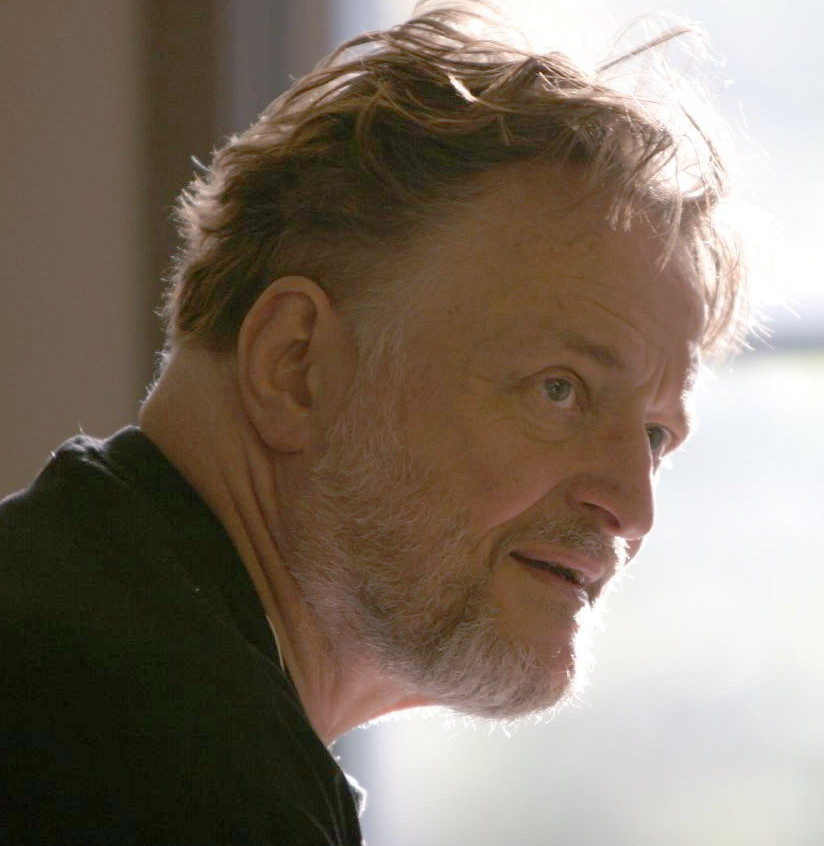
\includegraphics[width=0.9\textwidth]{conway} \\
		John H. Conway
% CC-BY: Thane Plambeck: http://www.flickr.com/photos/thane/20366806/
	\end{column}

	\begin{column}{0.5\textwidth}
		\centering
		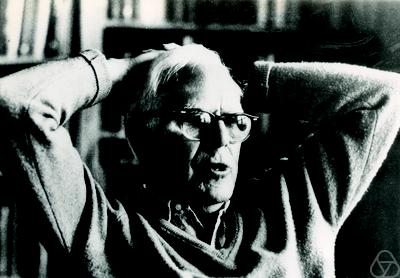
\includegraphics[width=0.9\textwidth]{gardner} \\
		Martin Gardner
% CC-BY-SA: http://owpdb.mfo.de/detail?photo_id=1292
	\end{column}
	\end{columns}
\end{frame}

\begin{frame}{The game of Life}
	\begin{itemize}
		\item From these simple rules, complicated and unpredictable behaviour arises
		\item We can make sense of the behaviour by looking at individual stable patterns
		\item Our aim will is to build up a pattern sufficiently complicated that it can compute
	\end{itemize}
\end{frame}

\begin{frame}{Some stable patterns}{Still lifes}
	\game{still1}{3}
	Still lives have period 1.
\end{frame}

\begin{frame}{Some stable patterns}{Still lifes}
	\game{beehive}{3}
	Still lives have period 1.
\end{frame}

\begin{frame}{Some stable patterns}{Blinkers}
	\game{blinker}{3}
	This blinker has period 2.
\end{frame}

\begin{frame}{More complex behaviour}{Gliders}
	\game{glider}{8}
	The glider shape has period 4, but moves from its original position.
\end{frame}

\begin{frame}{More complex behaviour}{Eaters}
	\game{eater}{6}
	The eater is a still life, but destroys a colliding glider in 4 turns.
\end{frame}

\begin{frame}{How complex can we go?}
	\begin{block}{Conjecture (Conway, 1970)}
		There does not exist an initial configuration such that the number of live cells after $n$ turns goes off to infinity.
	\end{block}
	\medskip

	\pause
	\begin{itemize}
		\item Disproved shortly afterwards
		\item In fact, a much more interesting result is true
	\end{itemize}
\end{frame}

\begin{frame}{More complex behaviour}{Glider guns}
	\imseq{Turn \n\\\medskip}{gosper}{0,3,6,...,42,45}
\end{frame}

\begin{frame}{How complex can we go?}
	\begin{block}{Theorem}
		Life is Turing-complete.
	\end{block}

	\pause
	\begin{center}
		\rotatebox{90}{$\iff$}
	\end{center}

	\begin{block}{Theorem}
		If anything else can compute the result of a given function, so can Life.
	\end{block}
\end{frame}

\begin{frame}{Logic gates}
	\begin{itemize}
		\item Many ways of modelling computation in Life have been discovered
		\item Modern digital computer chips are built from billions of logic gates
		\item Constructing logic gates in Life will give us a means to compute things
	\end{itemize}
\end{frame}

\begin{frame}{Logic gates}{NOT, AND and OR}
	\begin{itemize}
		\item Boolean functions operate on two values: on and off
		\item The most common gates are $\mathsf{NOT}$, $\mathsf{AND}$ and $\mathsf{OR}$
	\end{itemize}

	\bigskip
	\begin{columns}[onlytextwidth]
		\begin{column}{0.2\textwidth}
			\centering
			\begin{tabular}{c|c}
				$a$ & $\mathsf{NOT}~ a$ \\
				\hline
				\on & \off \\
				\off & \on
			\end{tabular}
		\end{column}

		\begin{column}{0.3\textwidth}
			\centering
			\begin{tabular}{c|c|c}
				$a$ & $b$ & $a ~\mathsf{AND}~ b$ \\
				\hline
				\on & \on & \on \\
				\on & \off & \off \\
				\off & \on & \off \\
				\off & \off & \off
			\end{tabular}
		\end{column}

		\begin{column}{0.3\textwidth}
			\centering
			\begin{tabular}{c|c|c}
				$a$ & $b$ & $a ~\mathsf{OR}~ b$ \\
				\hline
				\on & \on & \on \\
				\on & \off & \on \\
				\off & \on & \on \\
				\off & \off & \off
			\end{tabular}
		\end{column}
	\end{columns}

	\pause
	\medskip
	\begin{itemize}
		\item Any Boolean function can be expressed as a combination of these gates
	\end{itemize}
\end{frame}

\begin{frame}{Logic gates}{NAND}
	\begin{itemize}
		\item If we glue together an AND gate and then a NOT gate, we get a NAND gate
	\end{itemize}

	\begin{center}
		\begin{tabular}{c|c|c}
			$a$ & $b$ & $a ~\mathsf{NAND}~ b$ \\
			\hline
			\on & \on & \off \\
			\on & \off & \on \\
			\off & \on & \on \\
			\off & \off & \on
		\end{tabular}
	\end{center}

	\pause
	\begin{itemize}
		\item It turns out any Boolean function can be expressed as a combination of NANDs
		\item Even binary arithmetic can be done using Boolean functions
	\end{itemize}
\end{frame}

\begin{frame}{Bringing NAND gates to Life}
	\begin{itemize}
		\item Build a `circuit' where gliders act like electrons carrying current
		\item Just like in a real circuit, gliders present represents \on; no glider means \off
		\item We use glider guns as current sources
		\item To represent \off{} at a particular point, we use a stopper pattern to destroy the glider
	\end{itemize}
\end{frame}

\begin{frame}
\end{frame}

\end{document}
